Når temperaturen minker, vil K\textsubscript{2} øke ut i fra verdiene oppgitt i (tabell 4)(HENTET RETT FRA OPPGAVETEKST. MÅ FORANDRES). Da vil konsentrasjonen av CO\textsubscript{2} minke som igjen vil si at mer CO\textsubscript{2} vil gå over i gassfase. Dette vil igjen føre til at partialtrykket til CO\textsubscript{2} vil øke. Figur \ref{figurting} er et plot laget i Matlab for å illustrere.

\begin{figure}[H]  
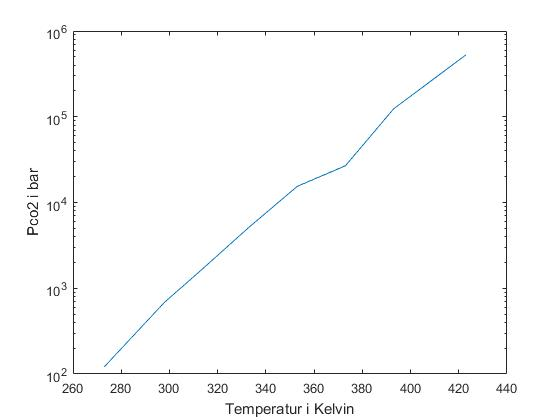
\includegraphics[scale=0.5]{Partialtrykkmottemp.jpg}
\centering
\caption{Partialtrykket til CO\textsubscript{2} i bar plottet mot temperatur med $\alpha=0.47$}
\label{figurting}
\end{figure}
